%%%%%%%%%%%%%%%%%%%%%%%%%%%%%%%%%%%%%%%%%
% Short Sectioned Assignment
% LaTeX Template
% Version 1.0 (5/5/12)
%
% This template has been downloaded from:
% http://www.LaTeXTemplates.com
%
% Original author:
% Frits Wenneker (http://www.howtotex.com)
%
% License:
% CC BY-NC-SA 3.0 (http://creativecommons.org/licenses/by-nc-sa/3.0/)
%
%%%%%%%%%%%%%%%%%%%%%%%%%%%%%%%%%%%%%%%%%

%----------------------------------------------------------------------------------------
%	PACKAGES AND OTHER DOCUMENT CONFIGURATIONS
%----------------------------------------------------------------------------------------

\documentclass[paper=a4, fontsize=11pt]{scrartcl} % A4 paper and 11pt font size

\usepackage[T1]{fontenc} % Use 8-bit encoding that has 256 glyphs
%\usepackage{fourier} % Use the Adobe Utopia font for the document - comment this line to return to the LaTeX default
\usepackage[english]{babel} % English language/hyphenation
\usepackage{amsmath,amsfonts,amsthm} % Math packages

\usepackage{lipsum} % Used for inserting dummy 'Lorem ipsum' text into the template

\usepackage{sectsty} % Allows customizing section commands
\allsectionsfont{\centering \normalfont\scshape} % Make all sections centered, the default font and small caps

\usepackage{fancyhdr} % Custom headers and footers
\pagestyle{fancyplain} % Makes all pages in the document conform to the custom headers and footers
\fancyhead{} % No page header - if you want one, create it in the same way as the footers below
\fancyfoot[L]{} % Empty left footer
\fancyfoot[C]{} % Empty center footer
\fancyfoot[R]{\thepage} % Page numbering for right footer
\renewcommand{\headrulewidth}{0pt} % Remove header underlines
\renewcommand{\footrulewidth}{0pt} % Remove footer underlines
\setlength{\headheight}{13.6pt} % Customize the height of the header

\numberwithin{equation}{section} % Number equations within sections (i.e. 1.1, 1.2, 2.1, 2.2 instead of 1, 2, 3, 4)
\numberwithin{figure}{section} % Number figures within sections (i.e. 1.1, 1.2, 2.1, 2.2 instead of 1, 2, 3, 4)
\numberwithin{table}{section} % Number tables within sections (i.e. 1.1, 1.2, 2.1, 2.2 instead of 1, 2, 3, 4)

\setlength\parindent{0pt} % Removes all indentation from paragraphs - comment this line for an assignment with lots of text

%----
%%Custom packages
%----
\usepackage{graphicx}

%----------------------------------------------------------------------------------------
%	TITLE SECTION
%----------------------------------------------------------------------------------------

\newcommand{\horrule}[1]{\rule{\linewidth}{#1}} % Create horizontal rule command with 1 argument of height

\title{	
\normalfont \normalsize 
\textsc{Technische Universit�t M�nchen, Lehrstuhl f�r Elektrische Antriebe und Leistungselektronik} \\ [25pt] % Your university, school and/or department name(s)
\horrule{0.5pt} \\[0.4cm] % Thin top horizontal rule
\huge Projekt: Identifikation eines Duffing Systems mit einem Neuronalen Netz \\ % The assignment title
\horrule{2pt} \\[0.5cm] % Thick bottom horizontal rule
}

\author{Maximilian Schermer, Matrikelnummer: 03664650, \\ Maximilian Sperr, Matrikelnummer: 03658841,\\ Giulio Evangelisti,  Matrikelnummer: 03659301} % Your name

\date{\normalsize\today} % Today's date or a custom date

\begin{document}

\maketitle % Print the title

%----------------------------------------------------------------------------------------
%	PROBLEM 1
%----------------------------------------------------------------------------------------
\newpage
\section{Duffing System}

System beschreiben, Simulationsergebnisse des Duffing Systems zeigen.

%------------------------------------------------

\section{Identifikationsmodell}\label{Identifikationsmodell}

Als Identifikationsmodell dient das General Dynamic Neuronal Network (GDNN) welches aus drei versteckten Schichten mit zweimal zwei und einmal einem Neuron (2-2-1) besteht. In der Eingangs sowie in der Ausgangsschicht befindet sich ein Neuron und die verschiedenen Schichten sind miteinander �ber Tapped Delay Lines gekoppelt. Die Tapped Delay Lines sind wie folgt aufgebaut:

\begin{table}[!h]
	\centering
		\begin{tabular}{*{3}{p{4cm}}}
			Schicht 1 & Schicht 2 & Schicht 3 \\
			$DI^{1,1} =  \left\{1,2,3\right\}$ & $DL^{2,1} =  \left\{0\right\}$ & $DL^{3,2} =  \left\{0\right\}$ \\
			$DL^{1,1} =  \left\{1,2,3\right\}$ & $DL^{2,2} =  \left\{1,2,3\right\}$ & $DL^{3,3} =  \left\{1,2,3\right\}$ \\
			$DL^{1,2} =  \left\{1,2,3\right\}$ & $DL^{2,3} =  \left\{1,2,3\right\}$ \\
			$DL^{1,3} =  \left\{1,2,3\right\}$ \\			
		\end{tabular}
\end{table}

Die Identifikation findet mittels eines NARX Modells statt, d.h. der Systemausgang und das Anregungssignal sind die Eing�nge f�r das neuronale Netz. Das GDNN wurde wegen seiner hohen Approximationsf�higkeit ausgew�hlt. 

Im folgenden wurde die zur Verf�gung gestellte Identifikationssoftware GDNN Version A verwendet.
%------------------------------------------------

\section{Systemanregung}

%Anregungssignal beschrieben, Grund f�r Chirp angeben, Frequenzabh�ngigkeit des Systems.
Wegen der starken Frequenzabh�ngigkeit unseres Systems, kann dieses nicht mit einem APRBS-Signal angeregt werden. Dies w�rde zu Amplitudenschwankungen des Systems f�hren welche den Lernprozess st�ren. Aus diesem Grund werden als Anregungssignal zwei Chirp Signale miteinander verbunden. Das erste Chirp Signale hat eine steigende Frequenz $\left[0; \frac{2}{\pi}\right]$ und das zweite eine abfallende Frequenz $\left[\frac{2}{\pi};0\right]$. Somit wird gew�hrleistet, dass alle Frequenzen bzw. Kreisfrequenzen $\left[0;4\right]$ der Frequenzantwort durchlaufen werden.
\begin{figure}[!h]
	\centering
		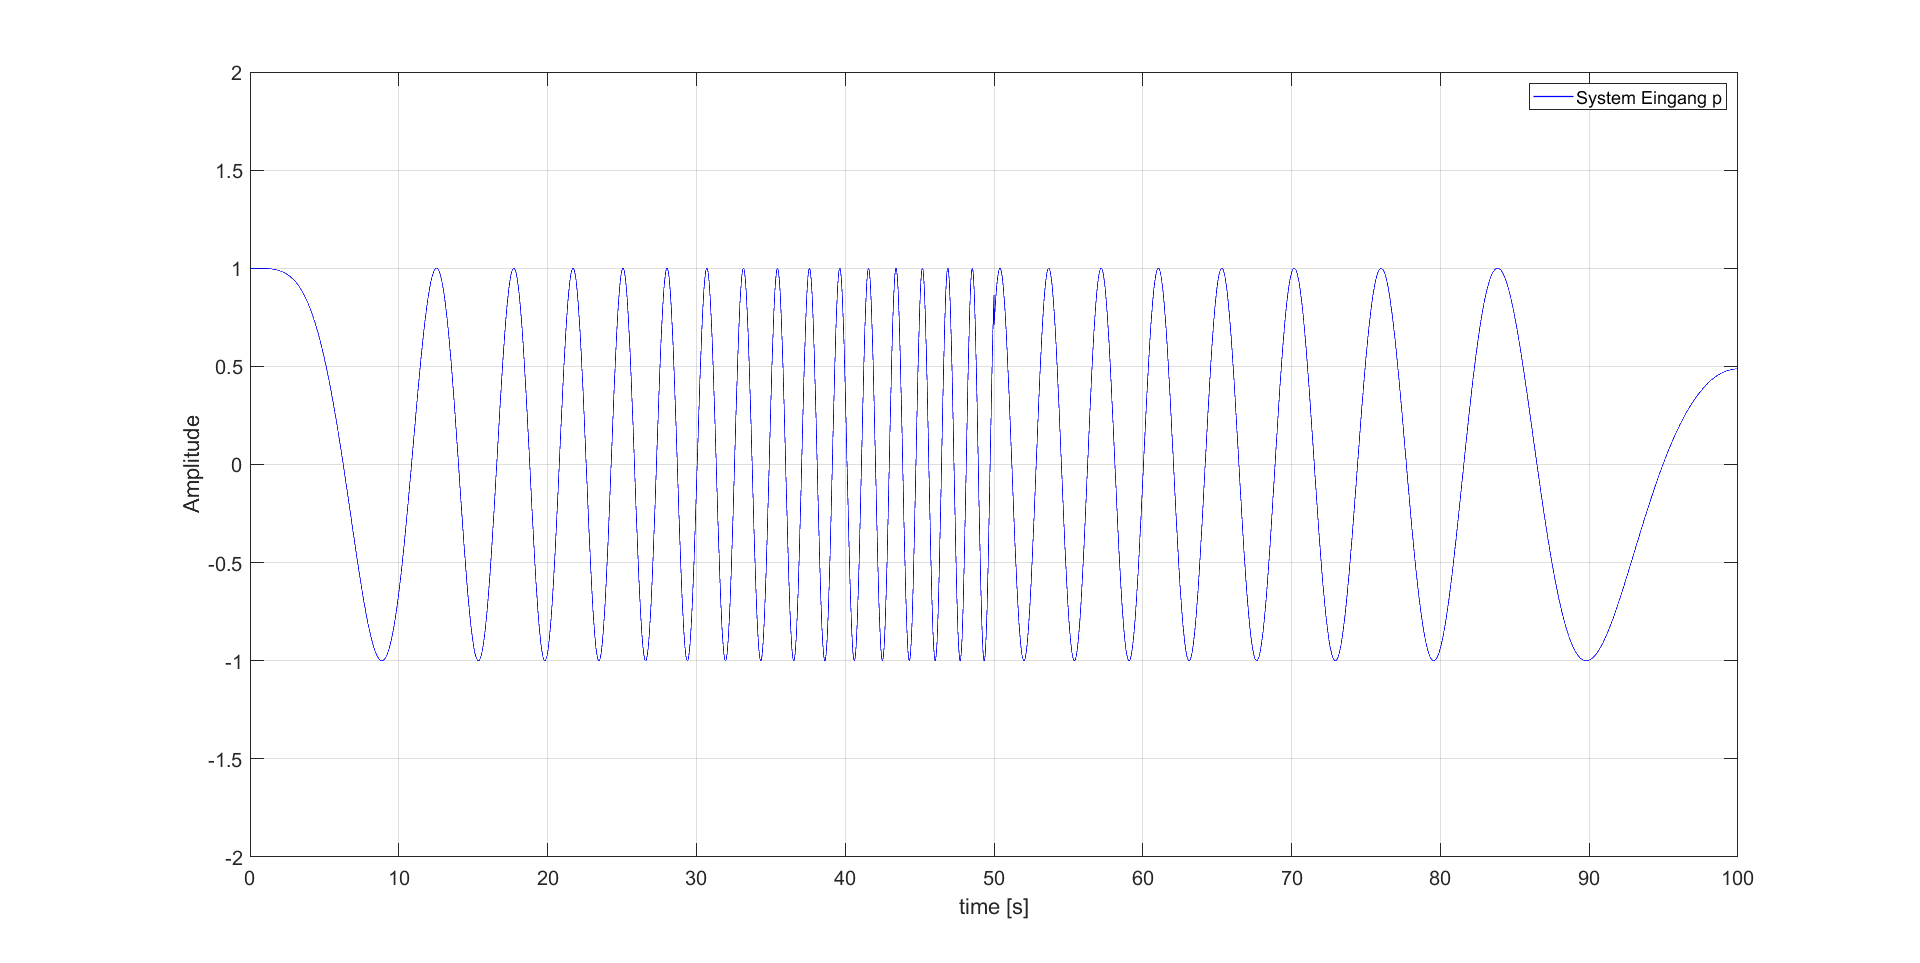
\includegraphics[width=0.55\textwidth]{./AnregungChirp.png}
	\caption{Anregungssignal}
	\label{fig:AnregungChirp}
\end{figure}
\newpage
%------------------------------------------------

\section{Identifikationsergebnisse}

%Identifikationsergebnis, Validierung Modell
Der Lernprozess wird �ber 100$s$ ausgef�hrt. Dabei ergeben sich folgende Identifikationsergebnisse:
Obwohl das System sehr starke Nichtlinearit�ten aufweist, erzielen wir gute Identifikationsergebnisse bis zu einem Fehler von $10^{-6}$. Dieses Ergebnis ist zufriedenstellend. Anfangs kommt es zu starken Abweichung, da der Lernprozess nicht weit fortgeschritten ist.
\begin{figure}[!h]
	\centering
		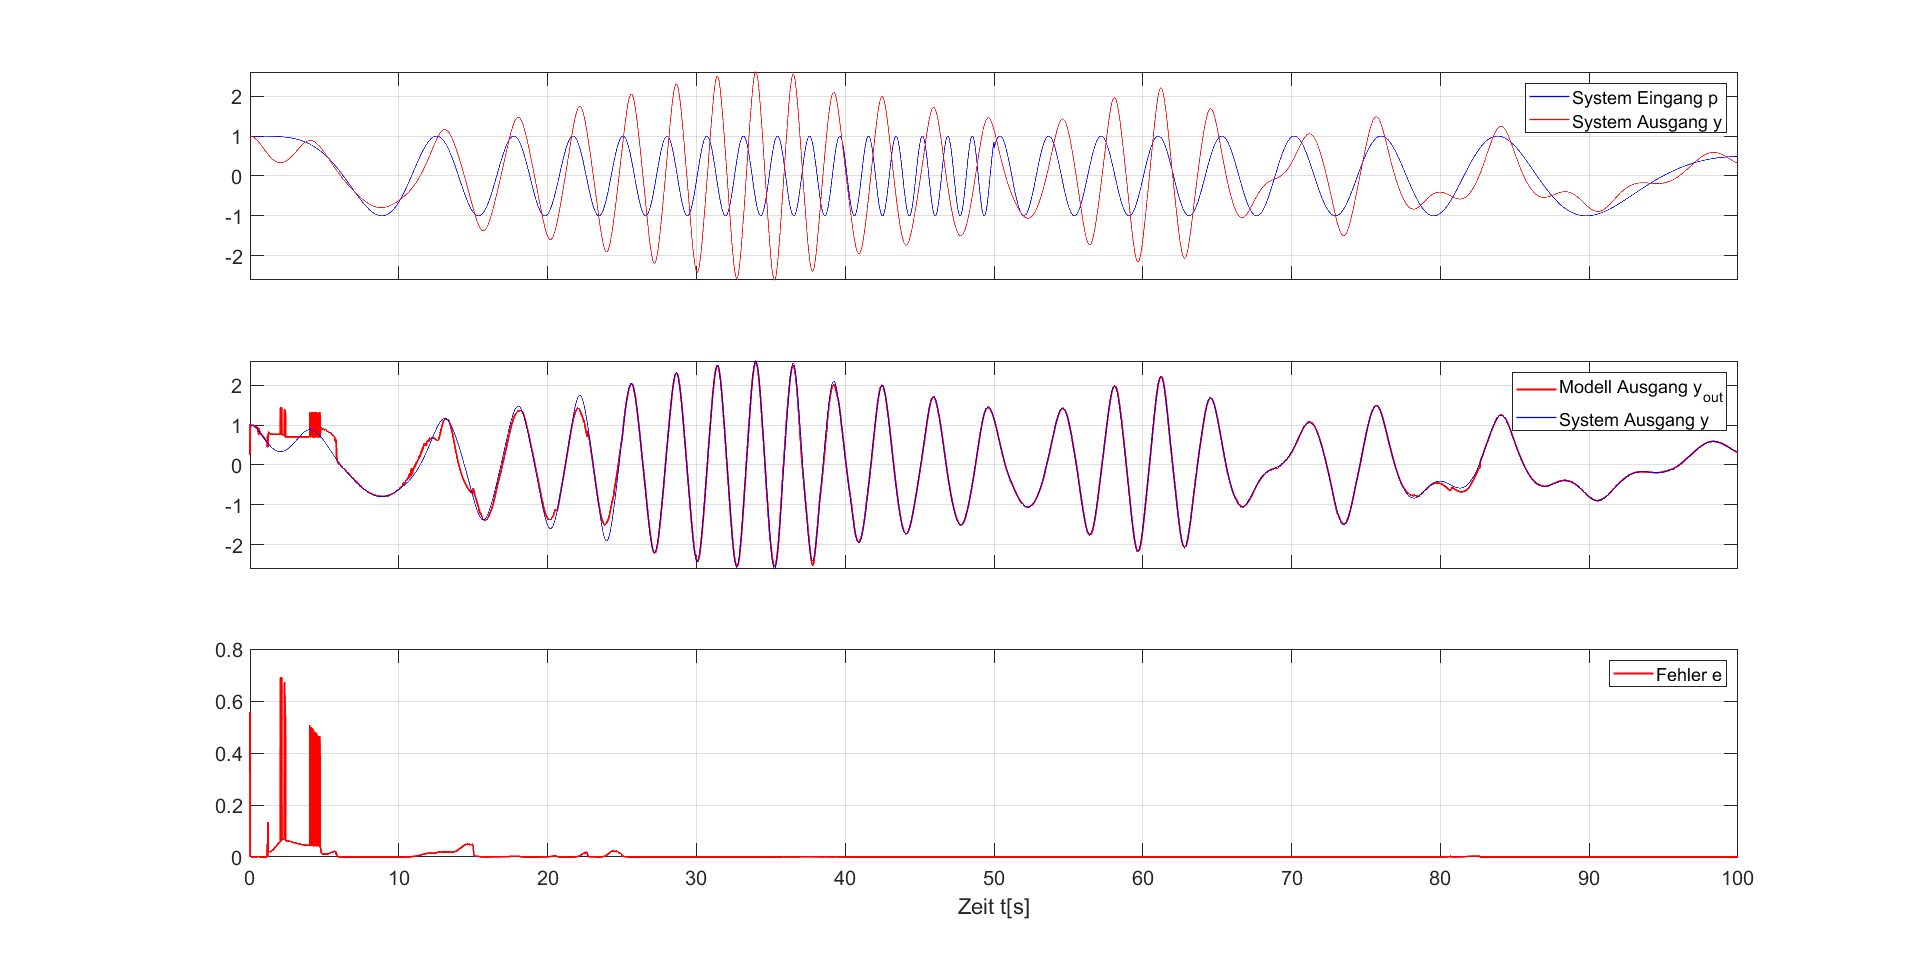
\includegraphics[width=1.00\textwidth]{./Q_500_nice_results_double_chirp.png}
	\caption{Anregungssignal, Ausgang System, Ausgang Modell}
	\label{fig:Nice_result_double_chirp}
\end{figure}

\begin{figure}[!h]
	\centering
		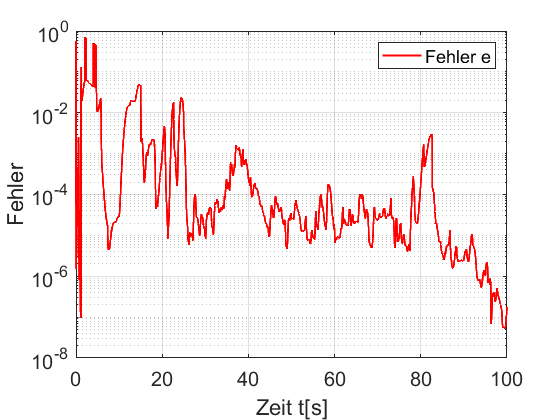
\includegraphics[width=0.5\textwidth]{./Q_500_nice_results_double_chirp_2.png}
	\caption{Verlauf des Fehlers}
	\label{fig:Nice_result_double_chirp2}
\end{figure}
\newpage

Eine erneute Identifikation �ber 80$s$ mit anschlie�ender Validierung �ber 20$s$, bei der der Lernprozess abgeschaltet wird, ergab folgende Ergebnisse: 
\begin{figure}[!h]
	\centering
		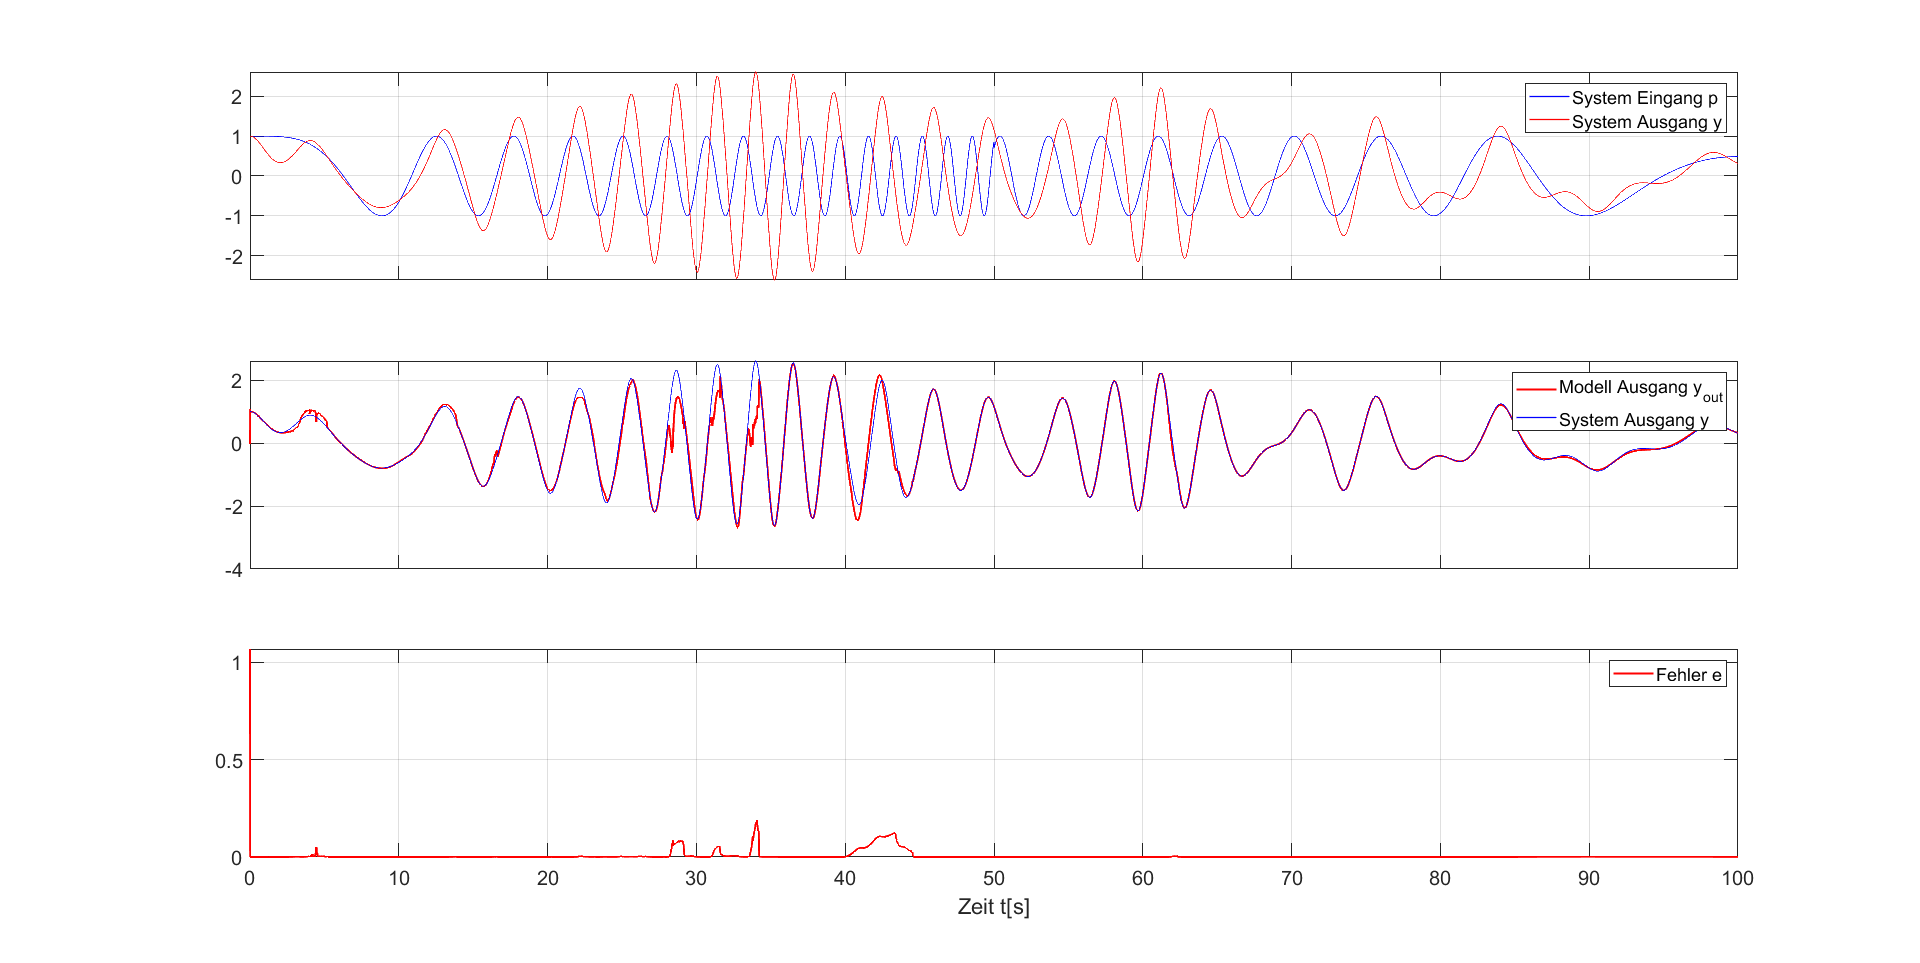
\includegraphics[width=1.00\textwidth]{./Q_500_nice_results_double_chirp_validierung_80.png}
	\caption{Anregungssignal, Ausgang System, Ausgang Modell mit Validierung nach 80s}
	\label{fig:Validierung}
\end{figure}

\begin{figure}[!h]
	\centering
		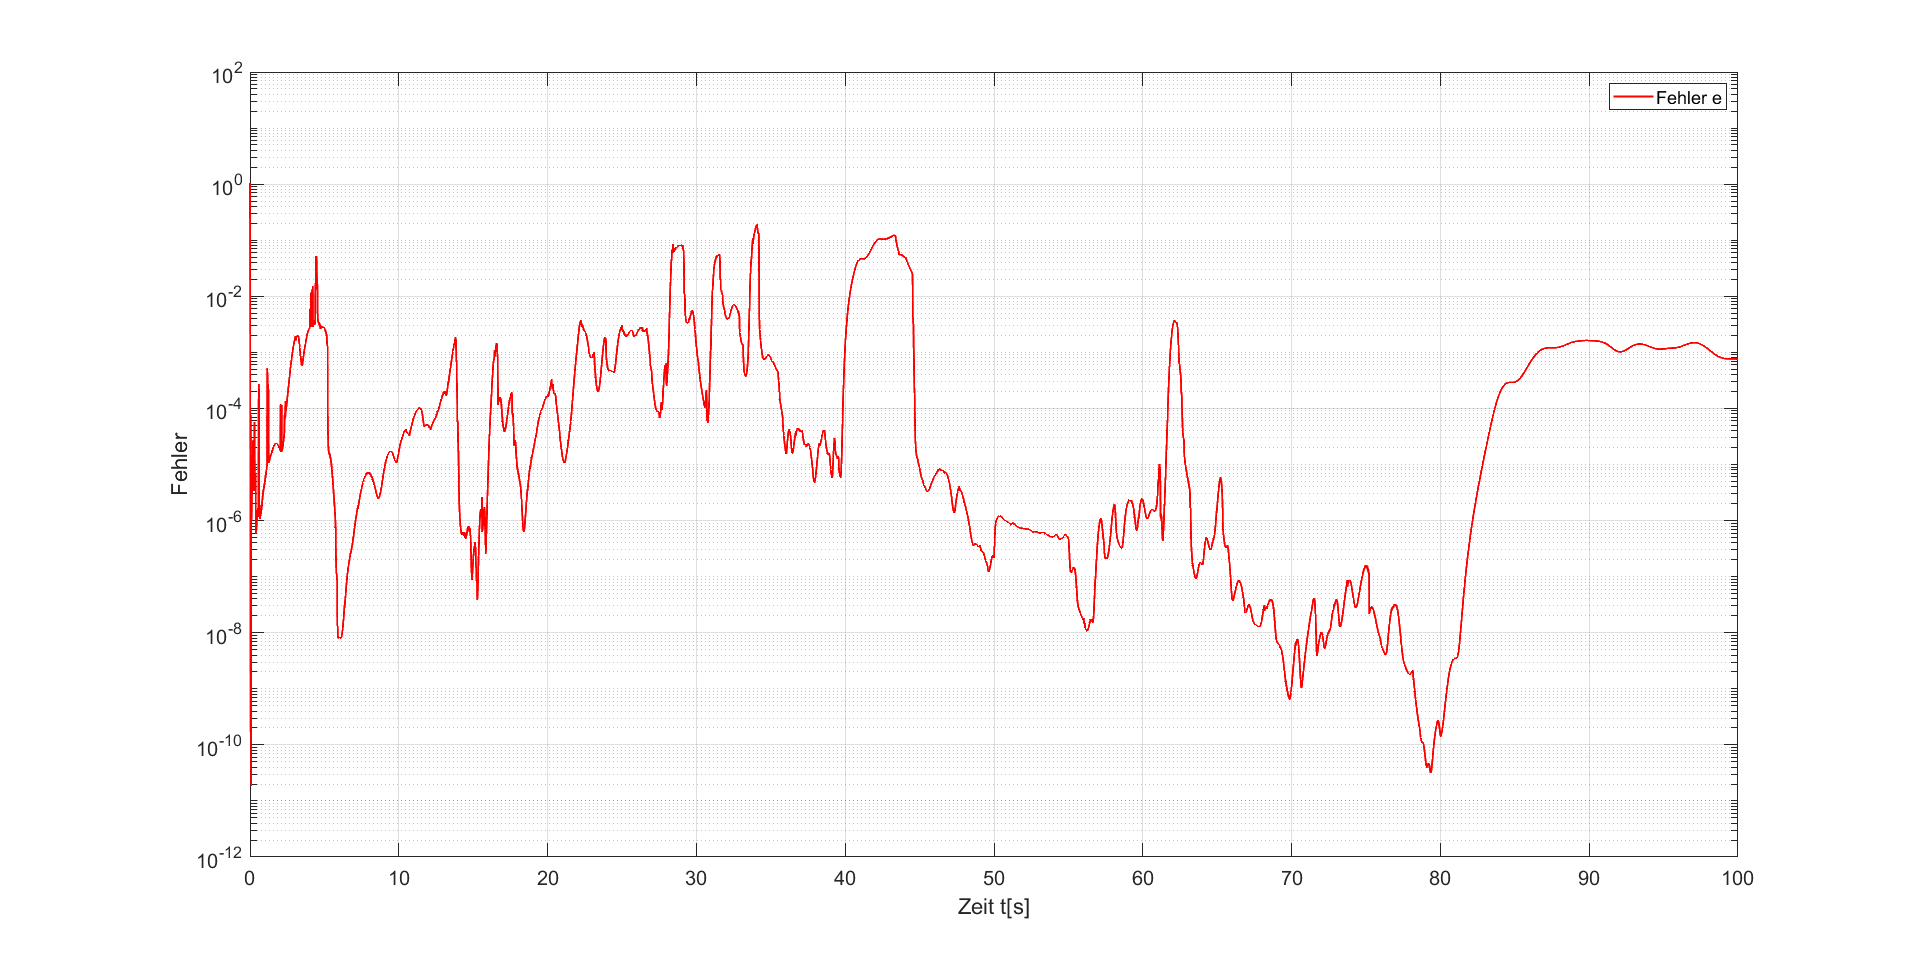
\includegraphics[width=0.5\textwidth]{./Q_500_nice_results_double_chirp_validierung_80_2.png}
	\caption{Verlauf des Fehlers mit Validierung nach 80s}
	\label{fig:Validierung2}
\end{figure}

Die Ergebnisse zeigen, dass der Fehler nach abschalten des Lernens zwar ansteigt, aber die Identifikation weiterhin gute Resultate liefert.
\newpage
%------------------------------------------------

\section{Anpassung des Identifikationsmodells}

%Modellstruktur und Anregungssignal �ndern. Zu statischen Identifikationsmodell wechseln.
\subsection{�nderung Modellstruktur}
Wird die Modellstruktur so abgewandelt, dass keine zeitliche Verz�gerungen (TDL) zwischen den Schichten existieren und die R�ckf�hrungen bestehen bleiben, so ergeben sich folgende Ergebnisse:
\begin{figure}[!h]
	\centering
		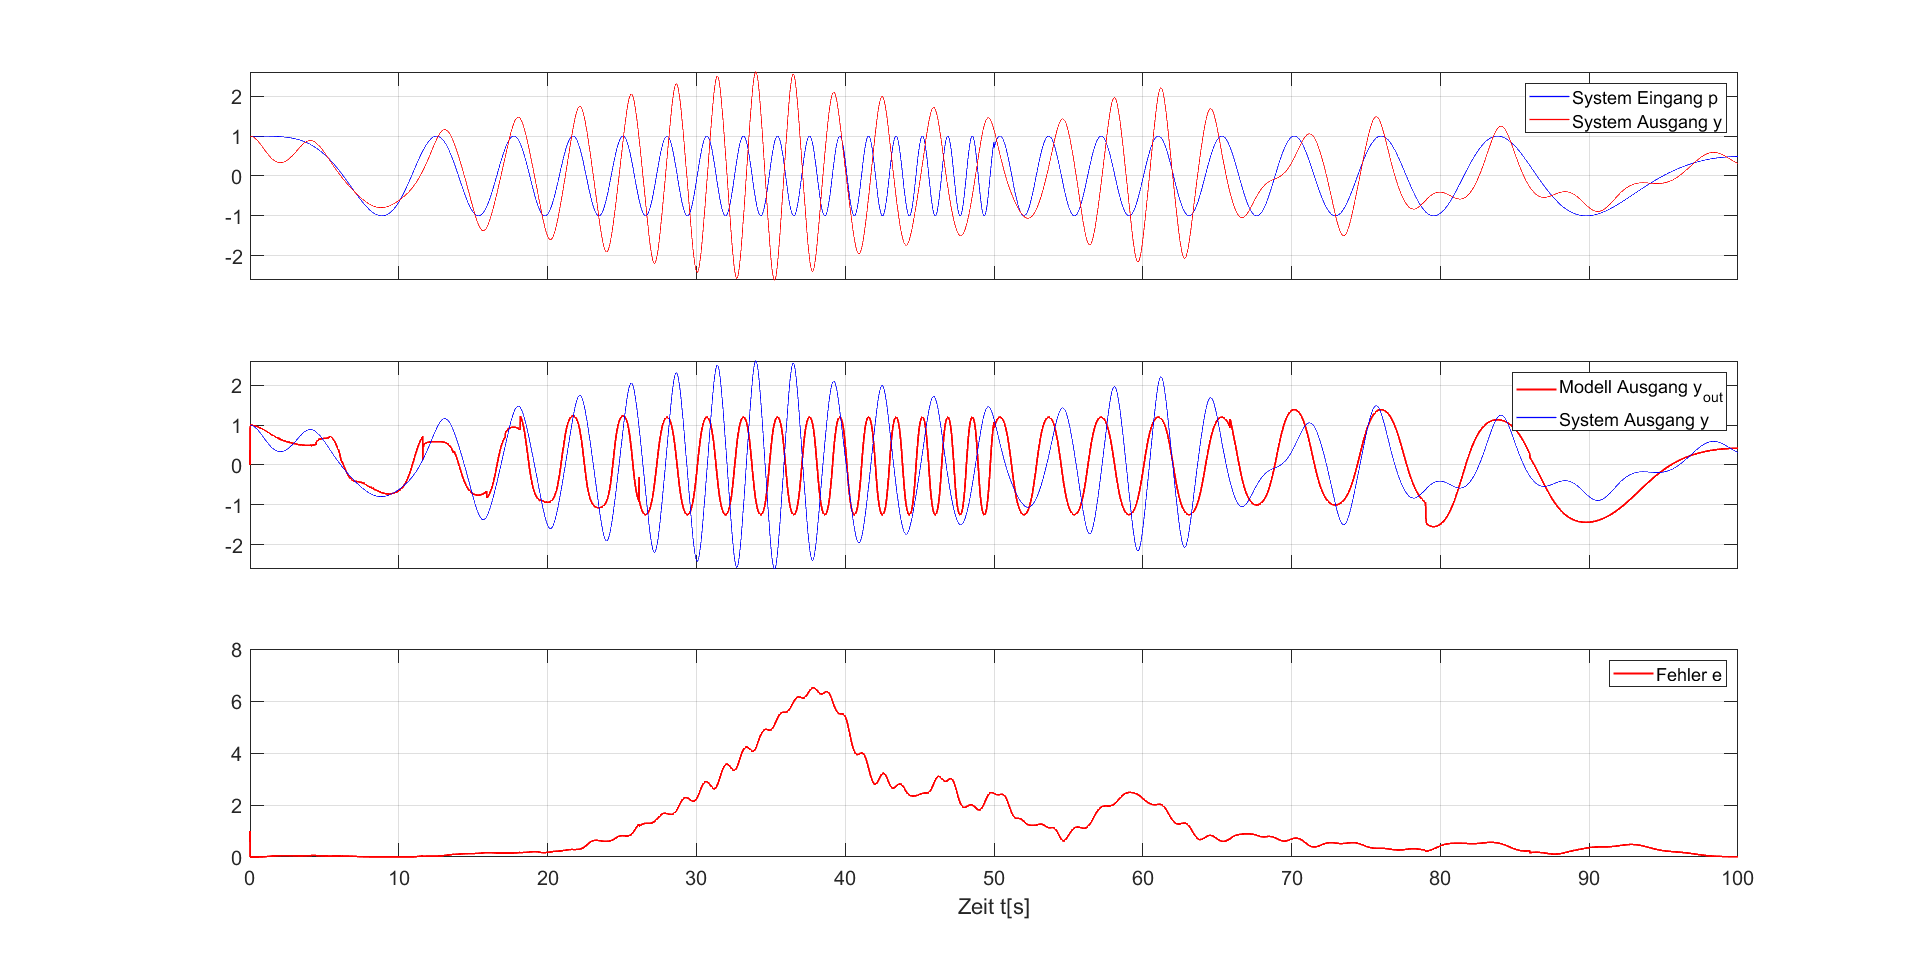
\includegraphics[width=1.00\textwidth]{./GDNN_ohneTDL_Identifikation.png}
	\caption{Anregungssignal, Ausgang System, Ausgang Modell mit GDNN ohne TDL}
	\label{fig:GDNN_ohneTDL}
\end{figure}

\begin{figure}[!h]
	\centering
		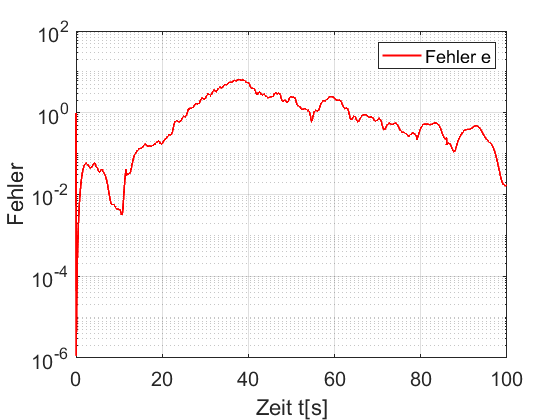
\includegraphics[width=0.5\textwidth]{./GDNN_ohneTDL_Identifikation_2.png}
	\caption{Verlauf des Fehlers mit GDNN ohne TDL}
	\label{fig:GDNN_ohneTDL2}
\end{figure}
\newpage

\subsection{�nderung Anregungssignal}
Eine �nderung des Anregungssignals auf ein klassisches APRBS Signal erzeugt den bereits schon angesprochene schlechten Lernprozess. Die Modellstruktur entspricht wieder der Struktur des zu Anfang angesprochene GDNN-Modells.
\begin{figure}[!h]
	\centering
		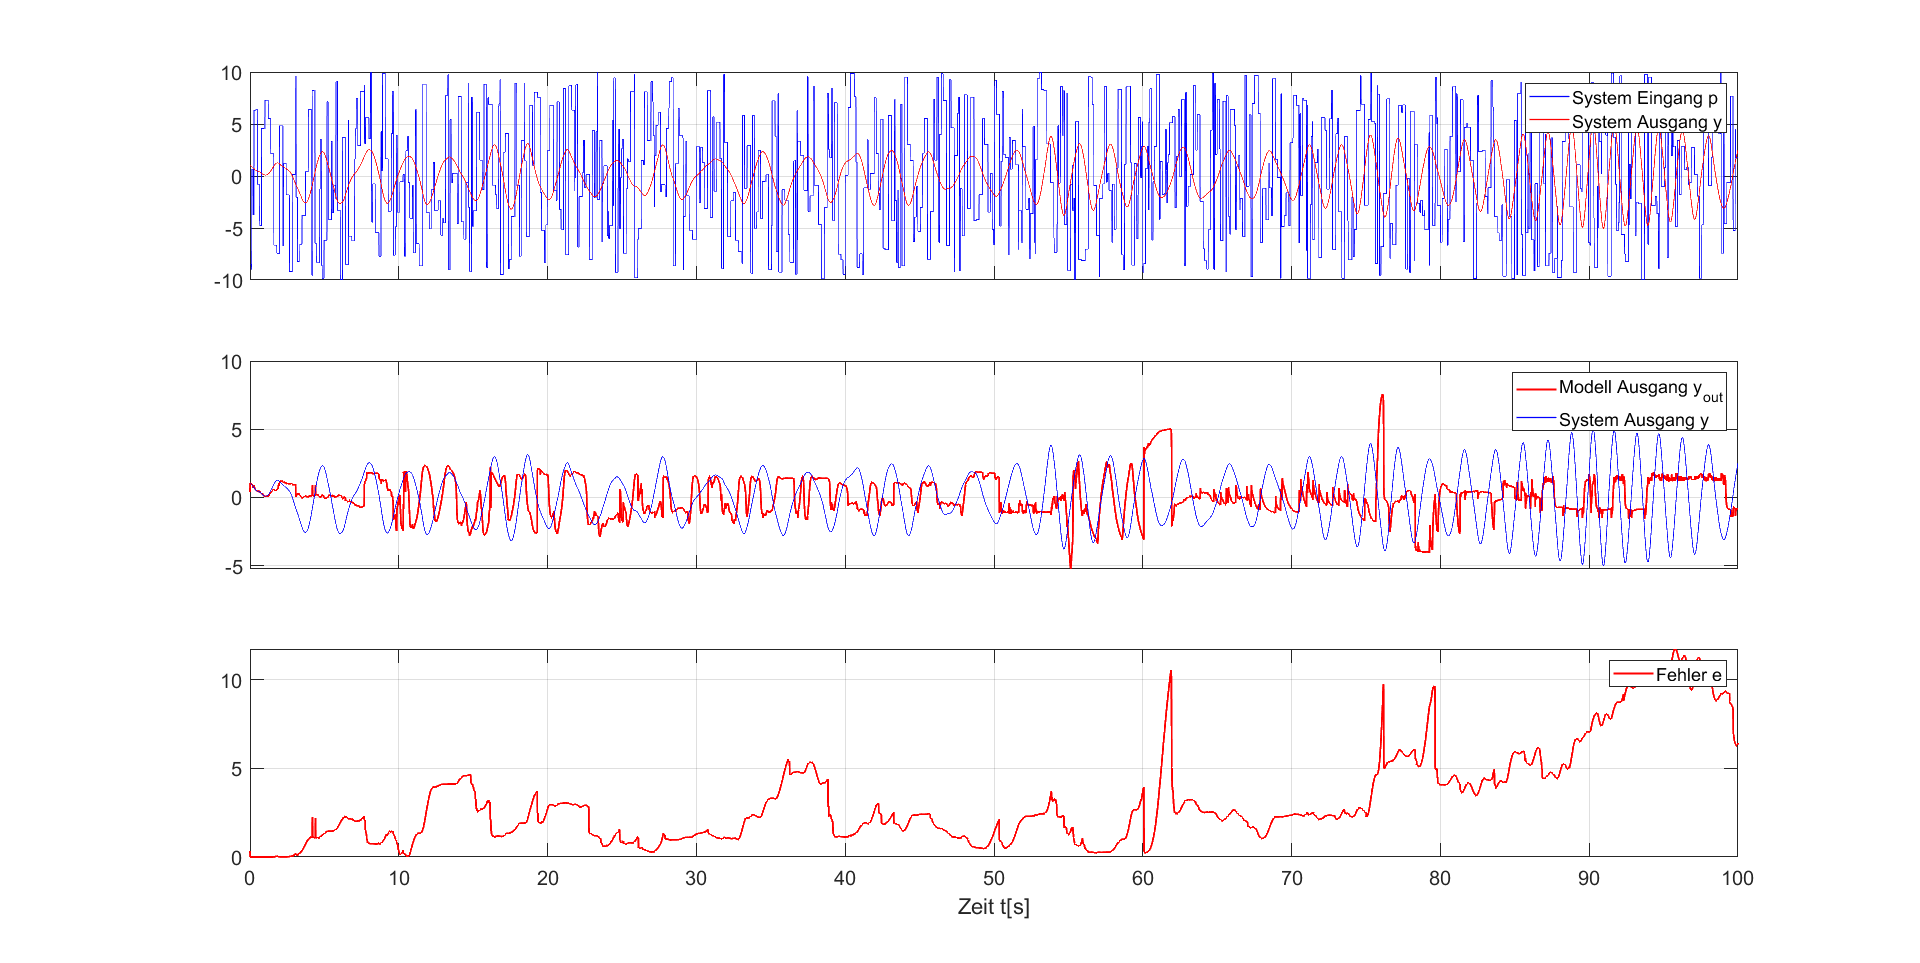
\includegraphics[width=1.00\textwidth]{./APRBS_GDNN.png}
	\caption{Anregungssignal, Ausgang System, Ausgang Modell mit APRBS-Signal}
	\label{fig:APRBS}
\end{figure}

\begin{figure}[!h]
	\centering
		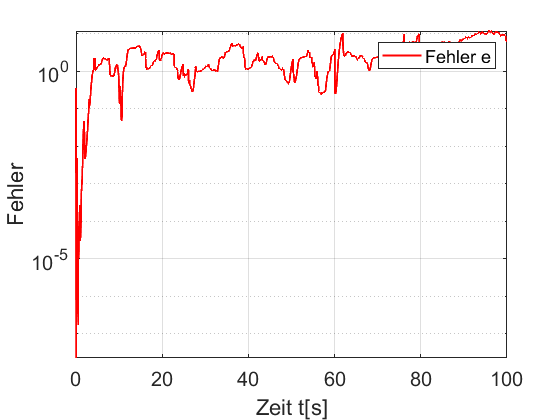
\includegraphics[width=0.5\textwidth]{./APRBS_GDNN_2.png}
	\caption{Verlauf des Fehlers mit APRBS-Signal}
	\label{fig:APRBS2}
\end{figure}
\newpage

\subsection{�nderung auf statisches Modell (MLP)}
Eine �nderung des Modells auf ein statisches Modell welches einem MLP entspricht, liefert ebenfalls einen schlechten Lernprozess. Dies liegt vor allem daran, dass das MLP die starke Nichtlinearit�t des Duffing Systems nicht identifizieren kann.
\begin{figure}[!h]
	\centering
		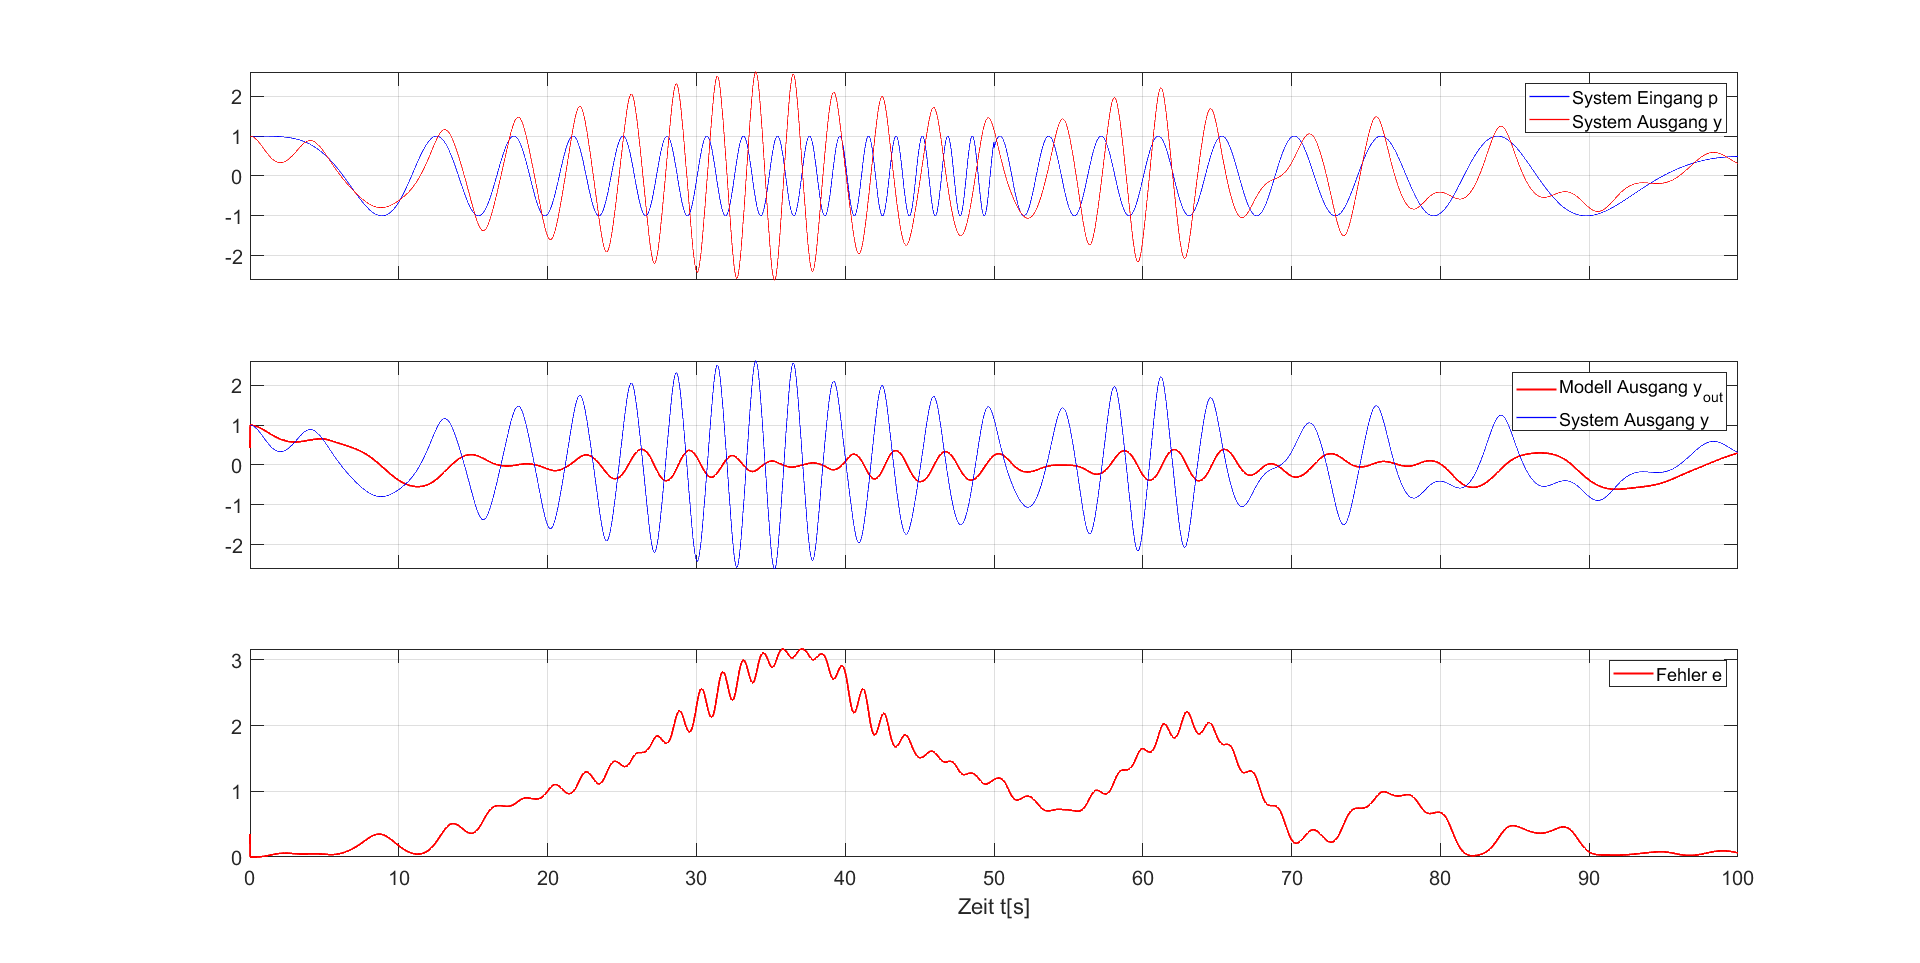
\includegraphics[width=1.00\textwidth]{./MLP_Identifikation.png}
	\caption{Anregungssignal, Ausgang System, Ausgang Modell mit MLP-Modell}
	\label{fig:MLP}
\end{figure}

\begin{figure}[!h]
	\centering
		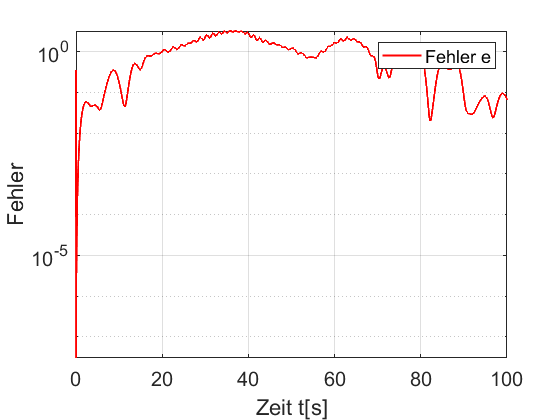
\includegraphics[width=0.5\textwidth]{./MLP_Identifikation_2.png}
	\caption{Verlauf des Fehlers mit MLP-Modell}
	\label{fig:MLP2}
\end{figure}
\end{document}